\chapter{Разработка новых алгоритмов формирования эталонов для автоматического распознавания речевых команд} \label{chapt2}

\section{Исследования статистических свойств используемых команд} \label{sect2_1}

Целью данного подраздела является оценка статистических свойств сигнала и результатов его частотно-временной параметризации.
Ключевое значение имеет исследование закона распределения и обоснование того, что во многих случаях это распределение для исследуемых параметров является нормальным.
Такая проверка необходима, так как подавляющее большинство применяемых алгоритмов используют гипотезу о нормальности.
Далее будет описан алгоритм проверки нормальности, а в следующем разделе приведены результаты проведённой практической проверки на имеющихся наборах данных.

%\newpage
%============================================================================================================================

\subsection{Проверка гипотезы о нормальности распределения отклонений элементов портрета слова от эталона} \label{sect2_1_1}

Пусть даны $M$ реализаций слова во временной области

\begin{equation} \label{eq:2_1_1_1}
\tilde{x}_k (t), \qquad k = 1, 2, \dots, M.
\end{equation}

Применяя алгоритм вычисления параметрического портрета слова, описанный в подразделе \ref{sect1_2_1}, получим для каждой реализации слова $\tilde{x}_k (t)$ параметрический портрет $X_k (i, j)$, представляющий собой матрицу, в которой строки $i = 1, 2, \dots, N_t$ соответствуют делению слова на $N_t$ интервалов по времени, а столбцы $j = 1, 2, \dots, N_f$ соответствуют частотным компонентам для каждого временного интервала.
По $M$ реализациям для каждого параметра $x_{ij}$ матрицы параметрического портрета можно рассчитать оценки математического ожидания, дисперсии и среднеквадратического отклонения по стандартным формулам выборочного оценивания:

\begin{equation} \label{eq:2_1_1_2}
\widehat{M}[x_{ij}] = \frac{1}{M} \sum_{k=1}^M X_k (i, j),
\end{equation}

\begin{equation} \label{eq:2_1_1_3}
\widehat{D}[x_{ij}] = \frac{1}{M - 1} \sum_{k=1}^M (X_k (i, j) - \widehat{M}[x_{ij}])^2,
\end{equation}

\begin{equation} \label{eq:2_1_1_4}
\widehat{\sigma}[x_{ij}] = \sqrt{\widehat{D}[x_{ij}]}.
\end{equation}

Для каждого элемента параметрического портрета каждого слова можно сформировать массив нормированных невязок

\begin{equation} \label{eq:2_1_1_5}
\Delta_{ij}^k = \frac{x_{ij}^k - \widehat{M}[x_{ij}]}{\widehat{\sigma}[x_{ij}]}, \quad
k = 1, 2, \dots, M, \quad
i = 1, 2, \dots, N_t, \quad
j = 1, 2, \dots, N_f,
\end{equation}
которые из определения имеют нулевое математическое ожидание и единичную дисперсию.
Данные величины будут проверяться на принадлежность к стандартному нормальному распределению, $\Delta_{ij}^k \in N(0, 1)$, что будет означать нормальность распределения отклонений элементов параметрического портрета слов от эталона.

Далее полученную матрицу невязок нужно перевести в набор из $M$ одномерных массивов $\epsilon^k (l)$, $k = 1, 2, \dots, M$, $l = 1, 2, \dots, N_t N_f$.
Для каждого одномерного массива можно применить критерий согласия Пирсона для проверки гипотезы о нормальности закона распределения, то есть гипотезы $H_0: \epsilon^k (l) \in N(0, 1)$ против гипотезы $H_1: \epsilon^k (l) \notin N(0, 1)$.
Результаты проверки описанной гипотезы о нормальности приведены в подразделе \ref{sect3_1_2}.

%\newpage
%============================================================================================================================

\subsection{Анализ влияния амплитуды слова на оцениваемые характеристики} \label{sect2_1_2}

Каждое слово записывается с разной амплитудой прежде всего из-за флуктуаций громкости произношения и изменения расстояния и ориентации губ диктора относительно микрофона.
Это означает, что уже во временной области каждая реализация имеет индивидуальный коэффициент усиления

\begin{equation} \label{eq:2_1_2_1}
c_k \tilde{x}_k (t), \qquad k = 1, 2, \dots, M.
\end{equation}

Оценим влияние разброса коэффициента усиления на результат вычисления среднего, то есть на эталон, по формуле \eqref{eq:2_1_1_2}.
Заметим, что элементы спектрального портрета $x_{ij}$, в соответствии с общепринятыми алгоритмами параметризации, описанными в подразделе \ref{sect1_2_1}, являются натуральными логарифмами оценок спектральных плотностей

\begin{equation} \label{eq:2_1_2_2}
x_{ij} = \ln(\widehat{S}_{ij}), \qquad \widehat{S}_{ij} = \tilde{F}_{ij} \tilde{F}_{ij}, 
\end{equation}
\begin{itemize}[align=left,leftmargin=1.8em,itemindent=0pt,labelsep=0pt,labelwidth=1.8em]
	\item[где] $\tilde{F}_{ij}$ --- результат дискретного преобразования $i$-го интервала времени и $j$-й частотной полосы после применения спектрального окна и усреднения по частоте.
\end{itemize}

Преобразование Фурье есть линейный оператор, поэтому

\begin{equation} \label{eq:2_1_2_3}
\tilde{F}_{ij} [c_k \tilde{x}_k (t)] = c_k \tilde{F}_{ij} [\tilde{x}_k (t)],
\end{equation}
то есть умножение исходной временной последовательности на постоянный коэффициент приводит к умножению результатов преобразования на этот же коэффициент.
Тогда для оценок спектральных плотностей получим 

\begin{equation} \label{eq:2_1_2_4}
\widehat{S}_{ij} [c_k \tilde{x}_k (t)] = c_k^2 \widehat{S}_{ij} [\tilde{x}_k (t)],
\end{equation}

Соответственно, для элемента параметрического портрета 

\begin{equation}
x_{ij} [c_k \tilde{x}_k(t)] =
\ln(c_k^2 \widehat{S}_{ij} [\tilde{x}_k]) =
2 \ln(c_k) + \ln(\widehat{S}_{ij} [\tilde{x}_k]),
\end{equation}
или

\begin{equation} \label{eq:2_1_2_5}
x_{ij} [c_k \tilde{x}_k(t)] =
2 \ln(c_k) + x_{ij} [\tilde{x}_k].
\end{equation}

Таким образом, умножение $k$-го слова на индивидуальный коэффициент усиления $c_k$ приводит к появлению в каждом параметре портрета дополнительного слагаемого $2 \ln(c_k)$, которое для $k$-го слова равно константе.
При вычислении оценки среднего \eqref{eq:2_1_1_2} по $M$ реализациям, получим

\begin{equation} \label{eq:2_1_2_6}
\begin{split}
\widehat{M} [x_{ij} [c_k \tilde{x}_k(t)]] = &
\frac{1}{M} \sum_{k=1}^M (2 \ln(c_k) + x_k(i,j)) = \\
= & \frac{1}{M} \sum_{k=1}^M 2 \ln(c_k) + \frac{1}{M} \sum_{k=1}^M x_k(i,j) =
c_M + \widehat{M} [x_{ij} [\tilde{x}_k(t)]].
\end{split}
\end{equation}

Итак, умножение каждого $k$-го слова на индивидуальный коэффициент приводит к появлению дополнительного слагаемого $c_M$, зависящего от $M$, которое добавляется к каждому элементу усреднённого параметрического портрета.
При фиксированном наборе реализаций $c_k \tilde{x}_k(t)$, $k = 1, 2, \dots, M$ величины $c_M = const$.
Разброс коэффициентов усиления $c_k$ должен привести к увеличению среднеквадратических отклонений параметров от среднего по ансамблю из $M$ реализаций.
Действительно, подставим в \eqref{eq:2_1_1_4} формулы \eqref{eq:2_1_2_5} и \eqref{eq:2_1_2_6}. Тогда,

\begin{equation} \label{eq:2_1_2_7}
\begin{split}
\widehat{\sigma^2} [x_{ij} [c_k \tilde{x}_k(t)]] = &
\frac{1}{M-1} \sum_{k=1}^M (x_{ij}[\tilde{x}_k(t)] + 2 \ln(c_k) - \widehat{M} [x_{ij}[\tilde{x}_k(t)]] - c_M)^2 = \\
= & \frac{1}{M-1} \sum_{k=1}^M ((x_{ij}[\tilde{x}_k(t)] - \widehat{M} [x_{ij}[\tilde{x}_k(t)]]) + (2 \ln(c_k) - \widehat{M}[2 \ln(c_k)]))^2,
\end{split}
\end{equation}
где учтено, что

\begin{equation} \label{eq:2_1_2_8}
c_M = \frac{1}{M} \sum_{k=1}^M 2 \ln(c_k) = \widehat{M}[2 \ln(c_k)].
\end{equation}

Раскроем в \eqref{eq:2_1_2_7} скобки, предполагая, что отклонение элементов портрета $x_{ij}$ от среднего не коррелированы с отклонениями логарифма коэффициента усиления $c_k$, и получим

\begin{equation} \label{eq:2_1_2_9}
\begin{split}
\widehat{\sigma^2} [x_{ij} [c_k \tilde{x}_k(t)]] \approx &
\frac{1}{M-1} \sum_{k=1}^M (x_{ij}[\tilde{x}_k(t)] - \widehat{M} [x_{ij}[\tilde{x}_k(t)]])^2 + \\
+ & \frac{1}{M-1} \sum_{k=1}^M (2 \ln(c_k) - \widehat{M}[2 \ln(c_k)])^2 =
\widehat{\sigma^2} [x_{ij}[\tilde{x}_k(t)]] + \widehat{\sigma^2} [2 \ln(c_k)].
\end{split}
\end{equation}

Выражение \eqref{eq:2_1_2_9} показывает, что наличие индивидуальных коэффициентов $c_k$ увеличивает оценку дисперсии элемента $x_{ij}$ по сравнению со случаем $c_k \equiv 1$.
Из \eqref{eq:2_1_2_9} следует, что при $c_k \ne 1$ формула \eqref{eq:2_1_1_4} даёт оценку суммы дисперсий двух случайных величин: элемента портрета $x_{ij}$ и удвоенного логарифма коэффициентов усиления $2 \ln(c_k)$.

Рассмотрим влияние индивидуальных коэффициентов усиления на результаты проверки гипотезы о нормальности отклонений элементов параметрического портрета от среднего.
Для случая $c_k \equiv 1$ отклонения от среднего задаются формулой \eqref{eq:2_1_1_5}.
При наличии индивидуальных для каждого слова коэффициентов усиления $c_k$ каждый член формулы \eqref{eq:2_1_1_5} изменяется.
При этом элемент параметрического портрета $x_{ij}^k$ определяется формулой \eqref{eq:2_1_2_5} и получает дополнительное приращение $2 \ln(c_k)$; среднее по ансамблю из $М$ реализаций изменяется согласно формуле \eqref{eq:2_1_2_6} и получает приращение $c_M = \frac{1}{M} \sum_{k=1}^M 2 \ln(c_k)$.
Наконец, оценка среднеквадратического отклонения элемента $\widehat{\sigma^2} [x_{ij}]$ по ансамблю из $М$ реализаций описывается формулой \eqref{eq:2_1_2_9} с дополнительным членом $\widehat{\sigma^2} [2 \ln(c_k)]$.
Все вышеперечисленные приращения являются константами и зависят или от отдельного значения коэффициента $c_k$ (формула \eqref{eq:2_1_2_5}), или от значений $c_k$ для всех $k = 1, 2, \dots, M$ (формулы \eqref{eq:2_1_2_6} и \eqref{eq:2_1_2_9}).
Это означает, что для элемента параметрического портрета при каждом значении $k$ отклонение от среднего $\Delta_{ij}^k$ уже не является случайной величиной с нулевым математическим ожиданием и единичной дисперсией, но имеет математическое ожидание и среднеквадратическое отклонение, индивидуальные для каждого значения $k$.

Таким образом, массив $\Delta_{k} (i, j)$, $k = 1, 2, \dots, M$ составлен из случайных величин с различными математическими ожиданиями и дисперсиями, хотя, возможно, имеющими нормальный закон распределения.
Такая композиция случайных величин в общем случае имеет распределение, отличное от нормального.
Поэтому для исключения влияния индивидуальных $c_k$ все $k = 1, 2, \dots, M$ слов следует привести к единому масштабу по амплитуде.

Для нахождения коэффициента коррекции по амплитуде для каждого слова используется следующая формула:

\begin{equation} \label{eq:2_1_2_10}
b_k^2 = \frac{E_{mean}}{E_k}\text{ , }k = 1, 2, \dots, M,
\end{equation}
где $E_{mean}$ --- средняя энергия сигнала по всем словам.

Для коррекции слова во временной области, умножим его на $b_k$

\begin{equation} \label{eq:2_1_2_11}
x_k(t)_{correct} = x_k(t) \cdot b_k.
\end{equation}

В итоге получается сигнал, скорректированный по амплитуде, для которого должны выполняться условия нормальности.

%\newpage
%============================================================================================================================

\subsection{Расчёт длительности слова, его энергии и средней частоты для различных дикторов} \label{sect2_1_3}

Для расчёта длительности слова в виде звукового сигнала $x(t)$ применяется формула

\begin{equation}
T = \frac{N}{Fs},
\end{equation}
\begin{itemize}[align=left,leftmargin=1.8em,itemindent=0pt,labelsep=0pt,labelwidth=1.8em]
	\item[где] $N$ --- число отсчётов в записи,
	\item[] $Fs$ --- частота дискретизации записи.
\end{itemize}

По $M$ реализациям записей одного слова можно получить оценки математического ожидания, дисперсии и среднеквадратического отклонения длительности слова.

Мгновенная мощность звукового сигнала задаётся формулой $p(t) = x^2 (t)$ \cite{max1983methods}.
Далее, энергия сигнала на некотором временном интервале $\Delta t$ в окрестности момента времени $t_0$ вычисляется по формуле

\begin{equation}
E(t_0, \Delta t) =
\int_{t_0 - \Delta t/2}^{t_0 + \Delta t/2} p(t) dt =
\int_{t_0 - \Delta t/2}^{t_0 + \Delta t/2} x(t)^2 dt.
\end{equation}

Полная энергия слова в форме дискретного сигнала выражение принимает следующий вид \cite{max1983methods}:

\begin{equation}
E(x) = \sum_{i=1}^{N} x_i^2,
\end{equation}
\begin{itemize}[align=left,leftmargin=1.8em,itemindent=0pt,labelsep=0pt,labelwidth=1.8em]
	\item[где] $N$ --- количество отсчётов в сигнале,
	\item[] $x_i$ --- амплитуда сигнала на $i$-м отсчёте.
\end{itemize}

Используя $M$ слов, можно посчитать среднее значение, дисперсию и среднеквадратическое отклонение энергии слова.

Также мощность сигнала может быть рассмотрена как функция от частоты $S(f)$.
Тогда она определяется как $S(f) = |X(f)|^2$, где $X(f)$ --- это фурье-образ функции $x(t)$.
В этом случае энергия сигнала в полосе частот от $f_0$ до $f_1$ определяется как

\begin{equation}
E(f_0, f_1) = \int_{f_0}^{f_1} S(t) df = \int_{f_0}^{f_1} |X(f)|^2 df.
\end{equation}

В качестве средней частоты принималась такая частота $f_{\text{ср}}$, что энергия составляющих сигнала с частотами в диапазоне $f \in [0, f_{\text{ср}}]$ равнялась энергии составляющих сигнала с частотами $f \in [f_{\text{ср}}, +\infty)$. Это эквивалентно условию

\begin{equation}
\int_{0}^{f_{\text{ср}}} S_x(f) df = \int_{f_{\text{ср}}}^{+\infty} S_x(f) df.
\end{equation}

Применяя быстрое преобразование Фурье (БПФ) можно получить оценки спектральных плотностей сигнала для дискретных значений частот $f_j$ в диапазоне $[0, 0.5 f_{\text{рег}}]$, где $f_{\text{рег}}$ --- частота регистрации сигнала: $\widehat{S}(f_j) = F(f_j) \cdot F^*(f_j)$, $j = 1, 2, \dots, \frac{N}{2}$, где $F(f_j)$ --- значение преобразования Фурье для частоты $f_j$.
Окончательно условие для определения средней частоты принимает вид:

\begin{equation}
\sum_{j=1}^{j_{\text{ср}}} \widehat{S}_x (f_j) \approx \sum_{j_{\text{ср}}+1}^{N/2} \widehat{S}_x (f_j).
\end{equation}

Таким образом получены формулы для расчёта длительности слова, его энергии и средней частоты.
Результаты вычислений описанных характеристик речевого сигнала и параметрических портретов показаны в подразделе \ref{sect3_1_2}.

%\newpage
%============================================================================================================================

\section{Разработка алгоритма разделения слов на фонетически однородные части на основе модифицированного метода динамического программирования} \label{sect2_2}

В естественной речи длительность произношения заданного слова, как и длительность каждого звука в слове, не является постоянной величиной.
Ручное выделение однородных частей в слове и их подстройка по времени позволяет улучшить результаты распознавания слов через их сравнение с эталоном.
Использование предварительной процедуры разбиения слова на однородные части является эффективным регуляризирующим фактором и позволяет уменьшить количество ошибок при распознавании \cite{savchenko2014algorithm}.
Поэтому данный алгоритм может применяться в любой процедуре распознавания, в которой присутствует сравнение с эталоном.
Но для эффективного алгоритма распознавания слов необходимо реализовать автоматический алгоритм разбиения слов на однородные части.

Предлагаемый способ предполагает автоматическое разделение слов на фонетически однородные части, определение границ которых осуществляется посредством решения задачи многопараметрической оптимизации.
При этом выдвигается предположение, что обеспечивается максимальная разнообразность фонетических показателей между смежными частями и максимальная однородность в рамках одной части.
Принятая мера степени различия и сходства основана на корреляции между столбцами матрицы параметрического портрета слова, получаемого в результате описанного в подразделе \ref{sect1_2_1} спектрально-временного преобразования аудиозаписи слова.
Интерес представляет то, что в ходе осуществлённых исследований был установлен факт того, что граница частей слов естественного языка рассчитывается в виде математической задачи на поиск экстремума.
Также, при разработке программно-аппаратного комплекса стоит уделить особое внимание временной сложности используемых алгоритмов, даже несмотря на рост производительности БЦВМ на летательных аппаратах.
Доработанный алгоритм на основе подхода динамического программирования предлагается в качестве способа для численного решения данной задачи.
Описание стандартного метода динамического программирования приведено в подразделе \ref{sect1_4_2}.

В данной части представлен сравнительный анализ различных методов, используемых при разбиении нескольких слов на однородные части с точки зрения близости автоматического и ручного разбиения слов.
В подразделе \ref{sect3_2} показаны результаты экспериментов, демонстрирующих корректность утверждённых допущений и способность предложенных алгоритмов решать поставленные задачи.

%\newpage
%============================================================================================================================

\subsection{Постановка задачи} \label{sect2_2_1}

Мотивацией для осуществления изложенных в работе исследований были следующие заключения:
\begin{enumerate}[label={\arabic*)}]
	\item Для передачи информации естественные языки, очевидно, используют собственный фонетический состав в качестве кода.
	Вследствие чего допустимо предположении о наличии аналогий между характеристиками слов и, к примеру, базовыми основами теории информации.
	\item Хорошо известно \cite{stratonovich1975theory}, что количественный показатель информации в сообщении обратно пропорционален количеству возможных версий самого сообщения.
	Из этого следует, что объём информации в сообщении тем больше, чем ниже вероятность его появления, то есть, чем менее оно похоже на другие возможные сообщения.
	Относительно звуков в словах естественных языков данный феномен можно трактовать таким образом, что объём информации в звуке тем больше, чем менее он созвучен другим звукам.
	И данный эффект характерен для всех звуков, содержащихся в слове, но наиболее ярко выражен для соседних звуков.
	Показатель разборчивости звуков и слов целиком в данном случае рассматривается в качестве меры количества информации.
	\item В естественных языках слова выработались в ходе длительного эволюционного процесса, ввиду чего они в некотором смысле оптимизированы.
	Ввиду чего возможно вынести предположение об оптимальности расположения границ между частями слова в рамках того или иного критерия.
	К примеру, необходимо создать условия максимальной разнородности соседних частей (звуков) и максимальную фонетическую однородность материала в рамках каждой части.
	В таком случае положение границ между частями слова возможно получить как решение математической задачей по нахождению экстремума.
\end{enumerate}

Интерпретируем эти общие рассуждения математически.
За основу принят параметрический портрет слова, представленный выше.
Следует помнить, что запись слова разделяется на $N_t$ простых равномерных временных отрезков по 10--30 мс каждый и вычисляются для 30--40 дискретных показателей частоты значения логарифмов оценок спектральных плотностей.
В качестве упрощения в рамках данного исследования используется равномерная шкала частот \cite{korsun2014algo, kolokolov2015compare}.
Применение логарифмических шкал мелов и барков, как показывает анализ, позволяет получить незначительное повышение качества распознавания \cite{korsun2014algo, kolokolov2015compare}.
Фонетически однородной частью, границы которой подлежат определению, назовём часть, содержащую два или более элементарных интервала.
Подобные части, как правило, соответствуют звуку, но в некоторых случаях могут соответствовать и слогу.
Очевидно, что число $L$ таких частей меньше числа элементарных интервалов, то есть $L < N_t$.
Выразим границы частей через номера интервалов $a_i$, $i = \overline{0, L}$, которые могут принимать значения $1 \le a_i \le N$.
Тогда для частей $k = \overline{1, L}$ границы задаются следующим образом:

\begin{equation} \label{eq:2_2_1_1}
\begin{gathered}
k = 1 : [a_0; a_1], \\
k = 2 : [a_1 + 1; a_2], \\
\dots \\
k = L : [a_{L-1} + 1; a_L],
\end{gathered}
\end{equation}
где $a_0 = 1$, $a_L = N$ и $a_1, a_2, \dots, a_{L-1}$ --- граничные интервалы частей.

Введённые границы \eqref{eq:2_2_1_1} означают, что часть 1 содержит интервалы от $1$ до $a_1$ включительно, часть 2 --- от $a_1 + 1$ до $a_2$ включительно и так далее.

Следует учесть, что столбцы матрицы параметрического портрета или вектора размерности 30--40, включающие логарифмы значений спектральных плотностей, соответствуют тому или иному элементарному временному интервалу.
В таком случае коэффициент корреляции между векторами двух элементарных интервалов будет являться мерой их близости.
Соответственно, для пары частей следует смотреть на средний коэффициент корреляции между элементарными интервалами, входящими в их состав.

Условием возможности разбиения слов на доли является их однородность в рамках каждой части и различие между собой смежных частей.
В терминах коэффициентов корреляции между элементарными интервалами это можно представить в виде следующих условий:
\begin{enumerate}[label={\arabic*)}]
	\item Интервалы, входящие в одну часть, должны иметь высокие коэффициенты корреляции между собой (однородность).
	\item Дисперсия взаимных коэффициентов корреляции между интервалами, входящими в одну часть, должна быть мала (однородность).
	\item Интервалы, входящие в одну часть, должны иметь малые коэффициенты корреляции с интервалами, входящими в соседние части (отличие).
\end{enumerate}

%\newpage
%============================================================================================================================

\subsection{Формирование критериев оптимизации} \label{sect2_2_2}

В качестве примера используем матрицу параметрического портрета слова со столбцами, соответствующими элементарным интервалам слова идентичной длительности, описание которой было дано выше.
Рассмотрим некоторую часть с номером $k$, содержащий интервалы с номерами от $a_{k-1} + 1$ до $a_k$.

В таком случае в виде верхней треугольной матрицы возможно отобразить между собой парные коэффициенты корреляции элементарных интервалов, являющихся составным элементом части.
Где в первой строке будут представлены коэффициенты корреляции параметрического портрета первого интервала с портретами последующих.
Соответственно, во второй строке следующие за вторым портреты будут коррелировать с параметрическим портретом второго интервала.
И дальнейшая структура матрицы будет построена по аналогии для всех остальных параметрических портретов интервалов всех частей.

Через среднее значение всех возможных пар коэффициентов корреляций внутри каждой части, можно интерпретировать условие 1, которое описывает однородность.
Найдём для каждой части оценки этого среднего:
\begin{equation}\label{eq:2_2_2_1}
\widehat{M}_k = \frac{1}{A_k} \sum^{a_k}_{i=a_{k-1}+1} \sum^{a_k}_{j=i+1} r_{ij},
\end{equation}
\begin{itemize}[align=left,leftmargin=1.8em,itemindent=0pt,labelsep=0pt,labelwidth=1.8em]
	\item[где] $A_k = \frac{1}{2} (a_k - a_{k-1})(a_k - a_{k-1} - 1)$ --- число попарных коэффициентов корреляции внутри части $k$, равное числу элементов соответствующей части $k$ верхней треугольной матрицы.
\end{itemize}

Очевидно, оптимальное разбиение слова на части, обеспечивающее их наибольшую однородность, должно соответствовать максимуму суммы оценок средних $\widehat{M}_k$ \eqref{eq:2_2_2_1} по всем $L$ частям слова:
\begin{equation}\label{eq:2_2_2_2}
\max_{a_0, a_1, \dots, a_L} \sum_{k=1}^L \widehat{M}_k.
\end{equation}

Для реализации условия 2, также характеризующего однородность, следует найти оценку дисперсий попарных коэффициентов корреляции внутри части:
\begin{equation}\label{eq:2_2_2_3}
\widehat{D}_k = \frac{1}{A_k-1} \sum^{a_k}_{i=a_{k-1}+1} \sum^{a_k}_{j=i+1} (r_{ij} - \widehat{M}_k)^2.
\end{equation}

Разбиение на части, оптимальное в смысле условия 2, должно обеспечивать минимум суммы дисперсий по $L$ частям:
\begin{equation}\label{eq:2_2_2_4}
\min_{a_0, a_1, \dots, a_L} \sum_{k=1}^L \widehat{D}_k.
\end{equation}

Критерии \eqref{eq:2_2_2_2} и \eqref{eq:2_2_2_4}, взятые по отдельности, могут соответствовать разным вариантам разбиения на части, хотя допустимо предположить, что результаты должны быть близкими.

Средний коэффициент корреляции между составляющими двух смежных частей $k$ и $k+1$ соответствует задающему различие условию 3:
\begin{equation}\label{eq:2_2_2_5}
\widehat{M}_{k,k+1} = \frac{1}{A_{k,k+1}} \sum^{a_k}_{i=a_{k-1}+1} \sum^{a_{k+1}}_{j=a_k+1} r_{ij},
\end{equation}
\begin{itemize}[align=left,leftmargin=1.8em,itemindent=0pt,labelsep=0pt,labelwidth=1.8em]
	\item[где] $A_{k,k+1} = (a_k - a_{k-1})(a_{k+1} - a_k)$ --- число элементов прямоугольной матрицы, содержащей взаимные коэффициенты корреляции между частями $k$ и $k+1$.
\end{itemize}

Очевидно, что чем меньше величина \eqref{eq:2_2_2_5}, тем сильнее отличие между частями.
Поэтому оптимальное разбиение должно удовлетворять критерию
\begin{equation}\label{eq:2_2_2_6}
\min_{a_0, a_1, \dots, a_L} \sum_{k=1}^{L-1} \widehat{M}_{k,k+1}.
\end{equation}

В общем случае результаты оптимизации разбиения по критериям \eqref{eq:2_2_2_2}, \eqref{eq:2_2_2_4} и \eqref{eq:2_2_2_6} могут не совпадать, хотя допустимо рассчитывать на близость результатов.
Для обеспечения возможности сравнения критериев \eqref{eq:2_2_2_2} и \eqref{eq:2_2_2_6} между собой суммы в этих формулах целесообразно заменить на среднее по числу частей:
\begin{equation}
J_1\{a_{0:L}\} = \frac{1}{L} \sum_{k=1}^{L} \widehat{M}_k,\qquad
J_2\{a_{0:L}\} = \frac{1}{L-1} \sum_{k=1}^{L-1} \widehat{M}_{k,k+1}.
\end{equation}

Кроме того, в критерии \eqref{eq:2_2_2_4} следует перейти к оценке среднеквадратического отклонения, чтобы все три критерия имели одинаковую размерность:
\begin{equation}
J_3\{a_{0:L}\} = \sqrt{\frac{1}{L} \sum_{k=1}^{L} \widehat{D}_k}.
\end{equation}

В качестве обобщённых критериев можно выбрать
\begin{equation}\label{eq:2_2_2_7}
J_{12}\{a_{0:L}\} = J_1\{a_{0:L}\} - J_2\{a_{0:L}\}
\end{equation}
или
\begin{equation}\label{eq:2_2_2_8}
J_{123}\{a_{0:L}\} = J_{12}\{a_{0:L}\} - \alpha_3 \cdot J_3\{a_{0:L}\},
\end{equation}
где $\alpha_3$ --- некоторый весовой коэффициент, подбираемый эмпирически.

Наиболее качественное разбиение определяется максимумом критериев \eqref{eq:2_2_2_7} или \eqref{eq:2_2_2_8}.
Метод перебора подходит для вычисления границ только небольшого количества частей, или, что то же самое, значений параметров $a_{0:L}$.

%\newpage
%============================================================================================================================

\subsection{Условия и порядок перебора} \label{sect2_2_3}

При решении оптимизационной задачи методом перебора задаются число частей и начальные значения пограничных точек, или узлов.
Значение шага интервала приравнивается к единице, соответствующей элементарному интервалу.
При переборе учитываются следующие правила:
\begin{enumerate}[label={\arabic*)}]
	\item точки $a_0$ и $a_L$ расположены в начале и в конце слова и считаются фиксированными;
	\item при переборе длина любого интервала не должна быть меньше $2$, то есть $a_{k+1} - a_k \ge 2$ при любых вариантах $k+1$ и $k$;
	\item приращения индексов составляют $\pm m$, то есть $k$-й узел может принимать значения $a_k = \{k_0 - m; k_0 - m + 1; \dots; k_0; k_0 + 1; \dots; k_0 + m\}$.
\end{enumerate}

Хотя в базовом варианте данная возможность и не была рассмотрена, также можно ввести зависимость величины приращения от номера узла $m = m_k$.
Выдвинутые выше критерии идентичности \eqref{eq:2_2_2_2} и \eqref{eq:2_2_2_4} бессмысленны в случае, если для приращения не соблюдается правило 2.
Поэтому оно обязательно должно выполняться.
Узлам присваиваются начальные значения перед началом процедуры перебора $a_k = k_0$, $k = \overline{0, L}$.

Учёт правила 2 осуществляется следующим образом.
Возьмём, например, три последних узла $a_{L-2}$, $a_{L-1}$, $a_L$, определяющих правые границы трёх последних интервалов с номерами $L-2$, $L-1$ и $L$.
Узел $a_L = L_0$ неизменен и соответствует концу слова.
Фиксируем начальное значение $a_{L-2} = (L-2)_0$ и задаём приращение узла $a_{L-1}$, при этом $a_{L-1} = (L-1)_0 \pm i$, $i = 1, 2, \dots, m$.
Для всех $i$ необходимо проверить оба неравенства: $a_L - a_{L-1} \ge 2$, $a_{L-1} - a_{L-2} \ge 2$.
Приращение в заданном направлении продолжается только в случае выполнения обоих условий.
Если нарушается первое условие, то прекращается увеличение $i$, если второе - прекращается уменьшение $i$.
После завершения циклов по $\pm m$ для $a_{L-1}$ задаётся приращение для узла $a_{L-2}$ и цикл $\pm m$ для $a_{L-1}$ повторяется.
Для каждого варианта индексов вычисляются значения критериев $J_1$, $J_2$, $J_3$.

Приращения задаются для всех $a_1, \dots, a_{L-1}$.
При небольшом числе узлов и малом диапазоне приращений задачу можно решить методом полного перебора.
Например, для девяти узлов, в каждом из которых проверяется три значения, общее число комбинаций равно $3^9 = 19683 \approx 2 \cdot 10^4$.
При девяти узлах для пяти значений в каждом общее число комбинаций равно $5^9 = 1953125 \approx 2 \cdot 10^6$.

Получается, что использование полного перебора практически возможно только при небольших приращениях индексов от начальных значений.
Для более точного разбиения слов на части потребуются очень большое время для работы алгоритма, поэтому целесообразно использовать методы динамического программирования, которые будут описаны в следующем подразделе.

%\newpage
%============================================================================================================================

\subsection{Практическое использование базовой схемы динамического программирования} \label{sect2_2_4}

В том случае, когда величина критерия рассчитывается для каждой части в отдельности, можно решить задачу с помощью существующих схем динамического программирования \cite{ventcel1980issledovanie}.
Для примера используем критерий $J_1$, тогда по формуле \eqref{eq:2_2_2_1} можно рассчитать значение среднего коэффициента корреляции между простыми интервалами каждой части.
Обозначим эти оценки средних коэффициентов $\rho_L$ для части $[a_{L-1} + 1; a_L]$, $\rho_{L-1}$ --- для части $[a_{L-2} + 1; a_{L-1}]$ и так далее (рисунок \ref{fig:dinprog_default}).

\begin{figure}[h]
	\centering
	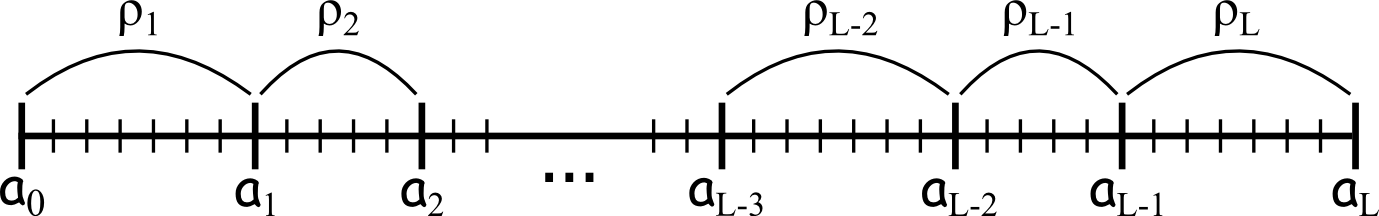
\includegraphics[width=15cm]{dinprog_default.png}
	\caption{Схема работы базового подхода динамического программирования}
	\label{fig:dinprog_default}
\end{figure}

Базовый подход работы данного алгоритма получается следующим.
Необходимо присвоить значения $a_{L-1}^j$, $j = \overline{-m, m}$ узлу $a_{L-1}$, в итоге, всего $2m+1$ значений.
Необходимо вычислить в части $[a_{L-1}^j + 1; a_L]$ оценку среднего коэффициента корреляции $\rho_L^j$ для всех $a_{L-1}^j$, что в сумме даст $2m + 1$ значений средних.
В данном случае, вследствие фиксации правой границы $a_L$, количество вариантов незначительно.
В итоге этого этапа фиксируются значения $a_{L-1}^j$ и соответствующие им оценки средних коэффициентов корреляции $\rho_L^j$, $j = \overline{-m, m}$.

Во время второго этапа изменениям подвергается граница $a_{L-2}$, расположенная слева, которой присваиваются значения $a_{L-2}^j$, $j = \overline{-m, m}$.
Но следует заметить, что в таком случае существует необходимость перебрать значения границы, расположенной справа $a_{L-1}^i$, $i = \overline{-m, m}$.
Для этого рассчитываются показатели оценок среднего коэффициента корреляции $\rho_{L-1}^{j, i}$, всего $(2m + 1)^2$ коэффициентов по количеству комбинаций для каждой конкретной комбинации $[a_{L-2}^j + 1; a_{L-1}^i]$.
В итоге каждому значению $a_{L-2}^j$ соответствует $2m + 1$ возможных положений границы $a_{L-1}^i$.
Из этих $2m + 1$ вариантов границ легко выбрать оптимальный в смысле максимума суммы оценок средних коэффициентов корреляции (далее для краткости суммарные оценки) в частях $[a_{L-2} + 1; a_{L-1}]$ и $[a_{L-1} + 1; a_L]$:
\begin{equation}
P_{L-1}^j = \max_{i} \{\rho_{L-1}^{j, i} + \rho_L^i \}.
\end{equation}

Итак, в результате второго этапа получены значения $a_{L-2}^j$ и соответствующие им суммарные оценки для двух крайних справа частей со значениями $P_{L-1}^j$.
Аналогично в результате третьего этапа получим для значений $a_{L-3}^j$ соответствующие им суммарные оценки для трёх крайних справа частей со значениями $P_{L-2}^j$, вычисляемыми по формуле
\begin{equation}
P_{L-2}^j = \max_{i} \{\rho_{L-2}^{j, i} + P_{L-1}^i \}.
\end{equation}

На предпоследнем этапе для узла $a_1$ получаем значения $a_1^j$ и выбираем оптимальный вариант, соответствующий максимальной суммарной оценке по всем частям:
\begin{equation}
P_1 = \max_{j} \{\rho_1^j + P_2^j \}.
\end{equation}

Рассмотренный алгоритм обеспечивает нахождение границ частей, оптимальных по критерию однородности $J_1$.
Для критерия $J_3$, также характеризующего однородность внутри части, задача решается аналогично. 

%\newpage
%============================================================================================================================

\subsection{Создание модифицированной схемы динамического программирования} \label{sect2_2_5}

Необходимость модификации стандартной модели обусловлена применением критерия, который зависит от обеих смежных частей с границами, заданными тремя узлами.
Предположим, что применяется составной критерий $J_{12}$, содержащий средние коэффициенты корреляции, как внутри одной части, так и между ними.
Рисунок \ref{fig:dinprog_modified} представляет границы частей и средние коэффициенты корреляции.

\begin{figure}[h]
	\centering
	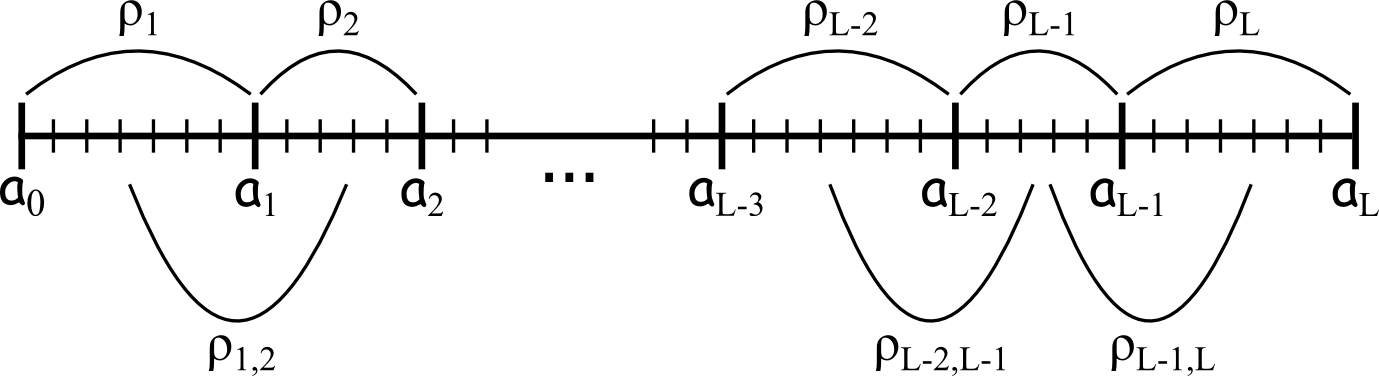
\includegraphics[width=15cm]{dinprog_modified.png}
	\caption{Схема работы предложенной модифицированной схемы динамического программирования}
	\label{fig:dinprog_modified}
\end{figure}

Здесь, в отличие от стандартной схемы, на каждом шаге следует перебирать значения не двух, а трёх узлов, то есть смотреть сразу на две части, что обусловлено взаимосвязью между смежными частями слов.

Был использован следующий доработанный алгоритм.
Во время первого этапа следует рассмотреть 2 крайние правые части.
Как и до этого, крайний узел $a_L$ принимается в качестве фиксированного.
Необходимо задать показатели приращения обеим другим узлам и перебрать все возможные сочетания положений границы $a_{L-1}^i$, $i = \overline{-m, m}$, $a_{L-2}^j$, $j = \overline{-m, m}$, что даёт $(2m + 1)^2$ комбинаций.
Оба изучаемых узла в полной мере задают значения двух крайних частей, находящихся справа, благодаря чему возможно рассчитать значение критерия $J_{12}$ для любого варианта их расположения.

Для проведения данной операции необходимо найти значение внутри всех частей $\rho_L^i$, $\rho_{L-1}^{j, i}$ и между частями $\rho_{L-1, L}^{j, i}$ средних коэффициентов корреляции для каждой пары индексов $i$ и $j$.
После чего для обеих частей $[a_{L-1} + 1; a_L]$ и $[a_{L-2} + 1; a_{L-1}]$ по формуле рассчитать средние коэффициенты корреляции (суммарные оценки):
\begin{equation}
P_{L-1, L}^{j, i} = \rho_L^i + \rho_{L-1}^{j, i} + \rho_{L-1, L}^{j, i}.
\end{equation}

Всего получаем $(2m + 1)^2$ значений суммарных оценок, которые приписываем каждой из $(2m + 1)^2$ комбинаций значений узлов $a_{L-1}^i$ и $a_{L-2}^j$.
В этом заключается результат первого этапа.
Во время второго этапа необходимо ввести узел $a_{L-3}$ и придать ему $2m + 1$ значений $a_{L-3}^l$, $l = \overline{-m, m}$.
Новый узел позволяет вычислить коэффициенты $\rho_{L-2}$ и $\rho_{L-2, L-1}$.
Эти коэффициенты, зависят также от значений границ предыдущей части, то есть от значений $a_{L-2}^j$ и $a_{L-1}^i$.
Используя эти значения и перебирая $(2m + 1)^3$ комбинаций по переменным $l$, $j$, $i$ вычисляем суммарные оценки
\begin{equation}
P_{L-2, L-1}^{l, j, i} = \rho_{L-2}^{l, j} + \rho_{L-2, L-1}^{l, j, i} + P_{L-1, L}^{j, i}.
\end{equation}

Итоговые количество рассчитанных значений равно $(2m + 1)^3$.
Выделим значения, соответствующие узлам $a_{L-3}$ и $a_{L-2}$, то есть индексам $l$, $j$.
У любой из комбинаций этих коэффициентов есть соответствующие $2m + 1$ значения узла $a_{L-1}$, или, что то же самое, индекса $i$.
Возьмём по индексу $i$ максимум.
В итоге получим $(2m + 1)^2$ значений суммарного коэффициента, соответствующую узлам $a_{L-3}$ и $a_{L-2}$:
\begin{equation}
P_{L-2, L-1}^{l, j} = \max_{i} \{ P_{L-2, L-1}^{l, j, i} \}.
\end{equation}

В результате второй этапа получим $(2m + 1)^2$ сочетаний коэффициентов $a_{L-3}$ и $a_{L-2}$.
При этом каждому из них будет приписана оптимальная по всем вероятным значениям узла $a_{L-1}$ величина совокупной оценки.
Соответственно, на предпоследнем этапе для узлов $a_1$ и $a_2$ количество значений составит $(2m + 1)^2$, которым по отдельности будет приписана оптимальная по всем доступным позициям узлов $a_3, \dots, a_{L-1}$ величина общей оценки:
\begin{equation}
P_{1, 2}^{k, j} = \max_{i} \{ P_{1, 2}^{k, j, i} \}.
\end{equation}

На последнем этапе добавляем узел $a_0$ и находим оптимальный вариант:
\begin{equation}
P_{1, 2} = \max_{l, j} \{ \rho_1^l + \rho_{1, 2}^{l, j} + P_{1, 2}^{l, j} \}.
\end{equation}

Таким образом, предложенная модифицированная схема метода динамического программирования является более сложной и требует перебора $(2m + 1)^3$ комбинаций вместо $(2m + 1)^2$ в стандартной схеме.
Обусловлено это тем, что вариант с модификациями соответствует критерию с введёнными составляющими, зависящими сразу от обеих смежных частей.
Ввиду этого необходимо углубить параметры перебора.

Результаты работы приведённых алгоритмов динамического программирования показаны в подразделе \ref{sect3_2}.

%\newpage
%============================================================================================================================

\section{Разработка алгоритма формирования эталонов на основе метода главных компонент} \label{sect2_3}

Представляется алгоритм оптимизации эталона, осуществляющий уменьшение размерности задачи оптимизации, посредством использования метода главных компонент.
Теоретическое описание метода главных компонент приведено в подразделе \ref{sect1_4_3}.

Формирование оптимального эталона заключается в разделении на главные компоненты и в последующей оптимизации коэффициентов разделения с помощью метода покоординатного спуска на обучающей выборке.
В представленном подразделе приведён алгоритм для получения оптимального эталона и описание способа расчёта главных компонент для рассматриваемой задачи.
Полученный в результате оптимизации эталон может быть применён в любых алгоритмах, которые используют сравнение с эталоном.
С целью снижения времени работы алгоритма рассматривается и метод его упрощения, при сохранении качества результатов.
Результаты тестирования, подтверждающие работоспособность предложенного подхода на примерах распознавания слов естественного русского языка с помощью новых эталонов представлены в подразделе \ref{sect3_3}.

%\newpage
%============================================================================================================================

\subsection{Описание алгоритма разложения спектрального портрета слова на главные компоненты} \label{sect2_3_1}

Пусть имеется $M$ параметрических портретов различных реализаций одного слова $X = \{x_{ij}(k)\}$, $k = 1, 2, \dots, M$; $i = 1, 2, \dots, N_t$; $j = 1, 2, \dots, N_f$.
Процедура формирования параметрических портретов слов подробно описана в подразделе \ref{sect1_2_1}.
Необходимо преобразовать матричный портрет для всех $k$ в одномерный массив с количеством элементов $l = 1, 2, \dots, P$, $P = N_f N_t$.
Итак, имеем $M$ векторов размерности $P$ каждый: $\{x_{lk}\}$, $k = 1, 2, \dots, M$; $l = 1, 2, \dots, P$.
В явном виде:

\begin{equation} \label{eq:2_3_1_1}
x_1 = \begin{bmatrix} x_{11} \\ x_{21} \\ \vdots \\ x_{P1} \end{bmatrix} \text{,  }
x_2 = \begin{bmatrix} x_{12} \\ x_{22} \\ \vdots \\ x_{P2} \end{bmatrix} \text{,  }
\dots
x_M = \begin{bmatrix} x_{1M} \\ x_{2M} \\ \vdots \\ x_{PM} \end{bmatrix} \text{,  }
\end{equation}

Объединим эти $M$ векторов в матрицу размерности $P \times M$:

\begin{equation} \label{eq:2_3_1_2}
X = \begin{bmatrix} x_1 & x_2 & \dots & x_M \end{bmatrix} = 
\begin{bmatrix}
x_{11} & x_{12} & \dots  & x_{1M} \\
x_{21} & x_{22} & \dots  & x_{2M} \\ 
\vdots & \vdots & \ddots & \vdots \\
x_{P1} & x_{P2} & \dots  & x_{PM} \\
\end{bmatrix}.
\end{equation}

Далее необходимо провести вычисление матрицы корреляционных моментов векторов $x_1, x_2, \dots, x_M$, имеющих размерность $M \times M$:

\begin{equation} \label{eq:2_3_1_3}
K_x = X^T X =
\begin{bmatrix} x_1^T \\ x_2^T \\ \vdots \\ x_M^T \end{bmatrix} \begin{bmatrix} x_1 & x_2 & \dots & x_M \end{bmatrix} = 
\begin{bmatrix}
x_1^T x_1 & x_1^T x_2 & \dots  & x_1^T x_M \\
x_2^T x_1 & x_2^T x_2 & \dots  & x_2^T x_M \\
\vdots    & \vdots    & \ddots & \vdots    \\
x_M^T x_1 & x_M^T x_2 & \dots  & x_M^T x_M \\
\end{bmatrix}.
\end{equation}

Заметим, что в матрице $K_x$ каждый элемент есть скалярное произведение соответствующих векторов и матрица $K_x$ симметричная.
Для неё можно вычислить $M$ собственных чисел $\lambda_1, \lambda_2, \dots, \lambda_M$ и соответствующих собственных векторов $l_1, l_2, \dots, l_M$ размерности $M$.
Собственные числа можно упорядочить по убыванию $\lambda_1 \ge \lambda_2 \ge \dots \ge \lambda_M$.

Определить первую главную компоненту $a_1$ необходимо как линейную комбинацию базовых векторов $x_1, x_2, \dots, x_M$, коэффициенты которых должны быть равны элементам их собственного вектора $l_1^T= [l_{11} l_{21} \dots l_{M1}]$:

\begin{equation} \label{eq:2_3_1_4}
a_1 = l_{11} x_1 + l_{21} x_2 + \dots + l_{M1} x_M = \sum_{i=1}^M l_{i1} x_i.
\end{equation}

Для главных компонент $m = 2, 3, \dots, M$ проводятся аналогичные расчёты по формуле:

\begin{equation} \label{eq:2_3_1_5}
a_k = \sum_{k=1}^M l_{km} x_k.
\end{equation}

В соответствии с теоретическими выкладками, представленными в подразделе \ref{sect1_2_2} сумма дисперсий исходных векторов и сумма дисперсий главных компонентов равны.
Таким образом, энергия сигналов при преобразование не изменяется.
Значение дисперсии главной компоненты $a_j$ равняется собственному числу $\lambda_j$.
Взаимная ортогональность является важным свойством главных компонент.
Целесообразность использования главных компонент заключается в наиболее существенном влиянии первых главных компонент на поведение системы $a_j$, $j = 1, 2, \dots, M'$.
Что делает возможным снизить размерность задачи и использовать $M'$ главных компонент вместо $M$ исходных векторов.
При необходимости оценить погрешность, связанную с переходом от $M$ изначальных векторов к $M'$ главным компонентам, можно воспользоваться величиной

\begin{equation} \label{eq:2_3_1_6}
I_p = \frac{\lambda_1 + \lambda_2 + \dots + \lambda_{M'}}{\lambda_1 + \lambda_2 + \dots + \lambda_M}.
\end{equation}

Как правило, первые несколько компонент содержат почти всю информацию о параметрическом портрете.
В подразделе \ref{sect3_3_1} будет определено количество главных компонент, которые несут существенную информацию о параметрическом портрете.
Также там будут приведены другие статистические расчёты, показывающие правильность работы метода главных компонент.

%\newpage
%============================================================================================================================

\subsection{Описание алгоритма формирования оптимизированных эталонов на основе метода главных компонент} \label{sect2_3_2}

Пусть эталоны для каждого из распознаваемых слов в словаре сформированы как усреднённый параметрический портрет всех реализаций.
Количественная оценка ошибок распознавания на выбранном диапазоне дикторов является наиболее простым способом оценки качества полученных эталонов.
Но при малом числе ошибок такая дискретная мера оценки качества распознавания не будет информативной и эффективной.
Поэтому целесообразно перейти к использованию некой непрерывной меры оценки качества распознавания.
Нижняя граница числового значения Z-преобразования Фишера коэффициента корреляции эталона с исследуемым словом может быть рассмотрена в виде такой непрерывной меры.
Просуммировав эти значения для каждого эталона, получим максимизируемую целевую функцию.

Другими словами, мера оценки качества распознавания трёх слов описывается следующей формулой:

\begin{equation} \label{eq:2_3_2_1}
F = \Delta Z^{low}_{1} + \Delta Z^{low}_{2} + \Delta Z^{low}_{3},
\end{equation}
где $\Delta Z^{low}_{i}$ определяется следующим образом:
\begin{equation} \label{eq:2_3_2_2}
\Delta Z^{low}_{i} = \min(\Delta Z_{ij}, \Delta Z_{ik}), \qquad i \ne j, i \ne k, j \ne k,
\end{equation}
а $\Delta Z_{ij}$ --- это разница Z-преобразований Фишера коэффициентов корреляций эталона $i$-го с распознаваемым $i$-м словом и эталона $j$-го с распознаваемым $i$-м словом.

Также можно дополнительно штрафовать за неправильное распознавание слова, что эквивалентно штрафу за значения $Z^{low}_{i}$ меньше нуля:

\begin{equation} \label{eq:2_3_2_3}
F = \Delta Z^{*low}_{1} + \Delta Z^{*low}_{2} + \Delta Z^{*low}_{3} \text{, где }
\Delta Z^{*low}_{i} = \left\{
\begin{array}{ll}
\Delta Z^{low}_{i}, \qquad\qquad\qquad \Delta Z^{low}_{i} \ge 0,\\
\Delta Z^{low}_{i} - \alpha (\Delta Z^{low}_{i})^2, \Delta Z^{low}_{i} < 0,
\end{array}
\right.
\end{equation}
где $\alpha$ --- это некоторое положительное число.

В формуле \eqref{eq:2_3_2_3} вместо нуля можно использовать любое другое положительно значение, которое будет интерпретироваться как зазор для устойчивости правильного распознавания.

Далее рассмотрим параметрический портрет эталона в виде линейной комбинации константы и $M'$ главных компонент с некоторыми коэффициентами: 

\begin{equation} \label{eq:2_3_2_4}
E_{syn} = k_0 a_0 + k_1 a_1 + \dots + k_{M'} a_{M'}.
\end{equation}

Задача получения оптимального эталона сводится к нахождению коэффициентов $k_0, \dots, k_{M'}$ таких, для которых должен выполняться критерий: $N_{ошибок} \rightarrow \min$, или величина Z коэффициента корреляции $\rightarrow \max$.
Подбор коэффициентов $k_0, \dots, k_{M'}$ можно произвести используя численные методы.

При построении $M'$ главных компонент может используется речевой материал нескольких дикторов.
Изначальное приближение коэффициентов рекомендуется выбирать из средних значений коэффициентов усреднённого эталона (выбранное как среднее из взятых эталонов) по результатам $M'$ главных компонент.
Дальнейшая оптимизация коэффициентов производится на обучающем наборе данных, который в общем случае может не совпадать с речевым материалом, по которому был получен эталон и начальное приближение коэффициентов.

В качестве метода оптимизации $F = f(k_0, \dots, k_{M'})$ выберем метод покоординатного спуска \cite{alekseeva2008, luenberger1984linear}.
Закон изменения коэффициентов разложения при $k_j > 0.001$: $k_{j+1} = k_j + l \Delta k_j$, $\Delta k_j = 0.01 |k_j|$, $l = 0, \pm 1, \pm 2, \pm 3, \pm 5, \pm 10, \pm 15, \pm 25, \pm 50, \pm 100, \pm 200$.
При условии $k_j \le 0.001$ применяется закон изменения с неизменным шагом: $k_{j+1} = k_j + 0.001 \Delta k_j$, $\Delta k_j = 0, \pm 1, \pm 2, \pm 3, \dots, \pm 10$.

Критерий остановки:
\begin{equation} \label{eq:2_3_2_5}
|F_{i+1} - F_i| \le \epsilon,\qquad \epsilon = 0.02 |F_i|.
\end{equation}

Другими словами, оптимизация завершается, когда значение оптимизируемой целевой функции изменяется меньше чем на 2~\%.
Независимый подбор коэффициентов для каждого слова является простым способом подбора, при котором коэффициенты разложения другой пары слов не меняются и остаются равными изначальному приближению.
В этом случае можно в качестве целевой функции использовать отдельные слагаемые из формул \eqref{eq:2_3_2_1} и \eqref{eq:2_3_2_3}.
Более сложный вариант заключается в оптимизации коэффициентов для каждого слова на каждой итерации оптимизационного процесса.
Тогда нужно использовать полную версию оптимизируемой целевой функции $F$.

В подразделах \ref{sect3_3_2} и \ref{sect3_3_3} будут приведены результаты оптимизации эталона с помощью предложенного метода, а также результаты распознавания слов оптимизированным эталоном.

%\newpage
%============================================================================================================================

\section{Разработка алгоритма формирования эталонов на основе полиномов Чебышёва} \label{sect2_4}

В данном подразделе рассматривается разработка алгоритма формирования эталонов на основе полиномов Чебышёва.
Теоретическое описание разложения произвольной функции на базис, образованный многочленами Чебышёва, дано в подразделе \ref{sect1_4_5}.

Пусть у нас есть параметрический портрет $X$, который содержит $N_f$ частотных полос и $N_t$ временных интервалов.
Данный параметрический портрет помимо самого речевого сигнала содержит ещё и неинформативные сигналы, обусловленные особенностями речи определённого диктора и шумами.
Использование полиномов Чебышёва поможет выделить только информативную часть, решив при этом сразу несколько задач.
Во-первых, это позволит уменьшить размерность параметрического портрета без существенной потери информативности, что упростит его хранение и ускорит обработку.
Вычислительная эффективность является одним из приоритетов разрабатываемых алгоритмов, поэтому ускорение обработки портретов является несомненным плюсом.

Во-вторых, выделение только самого речевого сигнала может помочь повысить качество распознавания.
При этом, можно проводить распознавание как сжатой версии параметрического портрета, так и восстановленной версии, которая не будет содержать лишних шумов.

Сжатие можно производить по частотным полосам, по временным интервалам и по обоим измерениям одновременно.
Для последнего случая получится сжатый параметрический портрет с $N'_f < N_f$ частотными полосами и $N'_t < N_t$ временными интервалами.
Суммарное количество элементов параметрического портрета уменьшится с $N_f \cdot N_t$ до $N'_f \cdot N'_t$.
Также возможно использование сжатие параметрических портретов с использованием полиномов Чебышёва не только для записей слов, но и для эталонов.

Результаты проверки сжатия параметрических портретов описаны в подразделе \ref{sect3_4}.

%\newpage
%============================================================================================================================

\section{Разработка алгоритмов формирования эталонов по нескольким дикторам на основе формулы Байеса и метода комитетов} \label{sect2_5}

Рассмотрена задача распознавания слов с использованием нескольких эталонов.
Общеизвестным фактом является то, что индивидуальные особенности диктора обуславливают параметры речи \cite{rabiner1993fundamentals, korsun2017recognition}.
Необходимо больше разнообразить речевой материал обучающей базы, с целью исключить дикторозависимость автоматического распознавания.
К примеру, можно использовать большее количество эталонов, при формировании которых применялись записи различных дикторов.

В данном подразделе предлагаются два алгоритма распознавания речевых команд с использованием нескольких эталонов. 
Первый алгоритм использует формулу Байеса \cite{ventcel1999theory}.
При данной методологии априорные условные вероятности гипотетических вариантов распознавания слов формируются на базе обучающей выборки, а затем найденные вероятности применяются при расчётах апостериорных вероятностей уже по факту получения результатов распознавания.
Благодаря этому удаётся повысить качество оценки, что, в свою очередь, положительно влияет на качество распознавания в условиях, когда невозможно произвести выбор состава команд.

В основе второго алгоритма лежит метод комитетов, в основе которого лежит независимое распознавание команд с помощью различных эталонов.
Данный алгоритм является модификацией стандартного метода комитетов, описанного в подразделе \ref{sect1_4_6}.
Всем возможным вариантам распознавания присваивается определённый балл.
В дальнейшем необходимо получить сумму полученных по всем эталонам баллов для формирования заключительной оценки, лежащей в основе определения результата распознавания.

Теоретическое обоснование представленных алгоритмов приведено ниже.
В данных алгоритмах для улучшения результатов распознавания могут быть применены подстройка по времени, описанная в подразделе \ref{sect2_2}, и оптимизированные эталоны, описанные в подразделе \ref{sect2_3}.
Также для ускорения работы алгоритмов может быть использовано сжатие используемых параметрических портретов, описанное в подразделе \ref{sect2_4}.
Для каждого из приведённых алгоритмов в подразделе \ref{sect3_5} представлены результаты экспериментальных исследований, подтверждающие их работоспособность.

%\newpage
%============================================================================================================================

\subsection{Алгоритм на основе формулы Байеса: определение задачи} \label{sect2_5_1}

В этом разделе также описывает решение задачи распознавания изолированных друг от друга команд.
Допустим, что в наличие есть гипотезы $H_1, H_2, \dots, H_M$ априорные вероятности которых составляют $P(H_1), P(H_2), \dots, P(H_M)$.
При распознавании им должны соответствовать $M$ различных слов.
В случае, когда по итогам распознавания принимается гипотеза $H_n$, можно сказать, что имело место событие $A_n$.
Предположим, что с целью распознавания получены $L$ разных эталонов, каждый состоящий из $M$ субэталонов, соответствующих отдельным словам.
Все субэталоны характеризует собой обобщённый параметрический портрет только одного слова из $M$ слов \cite{rabiner1993fundamentals, korsun2017recognition, korsun2016automatic}.
В основном, особенности всех $L$ эталонов обусловлены тем, что они составляются на базе речевого материала разных дикторов, ввиду чего и учитывают индивидуальные особенности его речи.
Тем не менее, вероятны и другие причины.

Распознавание по любому из $L$ эталонов производится путём последовательного вычисления скалярной меры близости $Z$ между параметрическим портретом распознаваемого слова и каждым из $M$ субэталонов.
Верной считается гипотеза, которая соответствует эталону слова с мерой близости $Z$, имеющей экстремум.
Традиционный порядок распознавания по единственному эталону соответствует этому \cite{rabiner1993fundamentals}.
В качестве меры близости может выбираться евклидово расстояние или расстояние Махаланобиса между векторами параметрического портрета \cite{rabiner1993fundamentals}, коэффициент корреляции \cite{korsun2016automatic}, Z-преобразование Фишера от коэффициента корреляции \cite{korsun2017recognition} и так далее.
Необходимо сформулировать задачу создания более качественной с математической точки зрения процедуры сравнения, позволяющей получить вероятностные оценки каждой гипотезы.
В первую очередь, это сделает возможным формирование иерархии наиболее вероятных гипотез даже после проведения процедуры распознавания с одним эталоном.
Кроме того, при использовании всех $L$ эталонов это позволит создать математически верный алгоритм для распознавания.
За основу возьмём формулу Байеса, используемую для вычисления апостериорных вероятностей \cite{ventcel1999theory}.
В первую очередь необходимо описать процедуру распознавания с использованием одного эталона.

Давайте предположим, что есть гипотезы $H_1, H_2, \dots, H_M$, которые соответствуют полной группе несовместных событий, характеризующихся значениями априорных вероятностей $P(H_1), P(H_2), \dots, P(H_M)$.
Пусть в результате распознавания по одному эталону произошло событие $A_k$, то есть принята гипотеза $H_k$.
В таком случае условная апостериорная вероятность любой из гипотез по формуле Байеса \cite{ventcel1999theory}, при выполнении условия наступления событий $A_{k_1}$, равняется:

\begin{equation}\label{eq:2_5_1_1}
P(H_i|A_k) = \frac{P(H_i) P(A_k|H_i)}{P(A_k)},
\qquad
i = 1, 2, \dots, M,
\end{equation}
\begin{itemize}[align=left,leftmargin=1.8em,itemindent=0pt,labelsep=0pt,labelwidth=1.8em]
	\item[где] $P(A_k|H_i)$ --- условная априорная вероятность события $A_k$ при условии, что верна гипотеза $H_i$.
\end{itemize}

Отметим, что событие $A_k$ может произойти только вместе с одним из событий $H_1, H_2, \dots, H_M$.
Тогда по формуле полной вероятности \cite{ventcel1999theory} вероятность события $A_k$ $P(A_k) = \sum_{j=1}^M P(H_j) P(A_k|H_j)$.

Подставляя в \eqref{eq:2_5_1_1}, получим другой вариант формулы Байеса, который и будем использовать в дальнейшем:

\begin{equation}\label{eq:2_5_1_2}
P(H_i|A_k) = \frac{P(H_i) P(A_k|H_i)}{\sum_{j=1}^M P(H_j) P(A_k|H_j)},
\qquad
i = 1, 2, \dots, M.
\end{equation}

Найти апостериорные вероятности любой гипотезы в условиях распознавания лишь по одному эталону можно по формуле \eqref{eq:2_5_1_2}.
Чтобы её было возможно применить, следует прежде оценить априорные вероятности гипотез $P(H_1), P(H_2), \dots, P(H_M)$, $i = 1, 2, \dots, M$, и найти для каждого события $A_k$ оценки априорных вероятностей событий $P(A_k|H_i)$, $k = 1, 2, \dots, M$, $i = 1, 2, \dots, M$.
Также требуется разработать алгоритм для подсчёта апостериорных вероятностей гипотез $H_i$ в условиях наличия производного количества эталонов.
Эти вопросы рассматриваются далее.

%\newpage
%============================================================================================================================

\subsection{Оценка априорных вероятностей экспериментальным методом} \label{sect2_5_2}

Формула Байеса \eqref{eq:2_5_1_2} включает априорные вероятности $P(H_i)$, $i = 1, 2, \dots, M$ каждой гипотезы.
Допускается давать им оценку равной вероятности, то есть $P(H_i) = 1/M$, а при многоэтапной процедуре распознавания --- исходить из апостериорной вероятности, основываясь на результатах предыдущего этапа.

Для применения формулы \eqref{eq:2_5_1_2} необходимо также получить оценки априорных условных вероятностей $P(A_k|H_i)$, $i = 1, 2, \dots, M$, то есть вероятностей события $A_k$ (вероятность признания гипотезы $H_k$ правильной) при условии, что верна гипотеза $H_i$, $i = 1, 2, \dots, M$.
С этой целью следует применить обучающую выборку.
Допустим, что обучающая выборка включает в себя $M$ слов по $E$ записей каждого.
В таком случае по итогам распознавания подсчитывается число событий $A_k$, $k = 1, 2, \dots, M$ для каждой гипотезы $H_i$, $i = 1, 2, \dots, M$.
Для нахождения оценки условных вероятностей можно использовать формулу:

\begin{equation}\label{eq:2_5_2_1}
P(A_k|H_i) = \frac{e_{ki}}{E},
\qquad
k = 1, 2, \dots, M,
\qquad
i = 1, 2, \dots, M,
\end{equation}
\begin{itemize}[align=left,leftmargin=1.8em,itemindent=0pt,labelsep=0pt,labelwidth=1.8em]
	\item[где] $e_{ki}$ --- число событий $A_k$ (верной признана гипотеза $H_k$), при условии, что верна гипотеза $H_i$.
\end{itemize}

Далее для расчёта апостериорных условных вероятностей $P(H_i|A_k)$ оценки, вычисленные по формуле \eqref{eq:2_5_2_1}, подставляются в \eqref{eq:2_5_1_2}.

%\newpage
%============================================================================================================================

\subsection{Методология расчёта апостериорных вероятностей гипотез в условиях применения более двух эталонов} \label{sect2_5_3}

Допустим, что исходно даны два эталона, используемых независимо друг от друга при распознавании.
В таком случае допускается использование формулы Байеса с целью определения показателей апостериорных вероятностей гипотез.
При двух эталонах следует рассматривать события $A_{k_1 k_2}$, соответствующие совместному распознаванию гипотез $H_{k_1}$ и $H_{k_2}$ по эталонам $C_1$ и $C_2$:

\begin{equation}\label{eq:2_5_3_1}
A_{k_1 k_2} = A_{k_1}^{C_1} A_{k_2}^{C_2},
\qquad
k_1 = 1, 2, \dots, M,
\qquad
k_2 = 1, 2, \dots, M,
\end{equation}
\begin{itemize}[align=left,leftmargin=1.8em,itemindent=0pt,labelsep=0pt,labelwidth=1.8em]
	\item[где] событие $A_{k_1}^{C_1}$ означает, что при распознавании по эталону $C_1$ верной признана гипотеза $H_{k_1}$,
	\item[] событие $A_{k_2}^{C_2}$ определено аналогично.
\end{itemize}

Событие $A_{kk}$ совпадения результатов распознавания по обоим эталоном является частным случаем \eqref{eq:2_5_3_1}.

\begin{equation}\label{eq:2_5_3_2}
A_{kk} = A_k^{C_1} A_k^{C_2}.
\end{equation}

Само собой, \eqref{eq:2_5_3_2} может быть выполнено в условиях корректного распознавания обоих эталонов, либо при совпадении их ошибок.

Условные вероятности события $A_{k_1 k_2}$ по гипотезам $H_i$ с учётом допущения о независимости распознаваний по эталонам 1 и 2

\begin{equation}\label{eq:2_5_3_3}
P(A_{k_1 k_2}|H_i) = P(A_{k_1}^{C_1}|H_i) P(A_{k_2}^{C_2}|H_i).
\end{equation}

При совпадении $k_1 = k_2 = k$ формула \eqref{eq:2_5_3_3} принимает вид

\begin{equation}\label{eq:2_5_3_4}
P(A_{kk}|H_i) = P(A_{k}^{C_1}|H_i) P(A_{k}^{C_2}|H_i).
\end{equation}

Условные вероятности событий $A_{k_1}^{C_1}$ и $A_{k_2}^{C_2}$ по гипотезам $H_i$ находятся отдельно для каждого эталона по обучающей выборке в соответствии с формулой \eqref{eq:2_5_2_1} предыдущего подраздела.

При двух эталонах формула Байеса \eqref{eq:2_5_1_2} принимает вид:

\begin{equation}\label{eq:2_5_3_5}
P(H_i|A_{k_1 k_2}) = \frac{P(H_i) P(A_{k_1 k_2}|H_i)}{\sum_{j=1}^M P(H_j) P(A_{k_1 k_2}|H_j)}.
\end{equation}

Для произвольного числа $L$ применяемых независимо эталонов рассмотрим событие

\begin{equation}\label{eq:2_5_3_6}
A_{k_1 k_2 \dots k_L} = A_{k_1}^{C_1} A_{k_2}^{C_2} \dots A_{k_L}^{C_L}
\end{equation}
и его частный случай

\begin{equation}\label{eq:2_5_3_7}
A_{kk \dots k} = A_{k}^{C_1} A_{k}^{C_2} \dots A_{k}^{C_L}.
\end{equation}

Формула \eqref{eq:2_5_3_4} для условных вероятностей события $A_{k_1 k_2 \dots k_L}$ при допущении о независимости эталонов принимает вид:

\begin{equation}\label{eq:2_5_3_8}
P(A_{k_1 k_2 \dots k_L}|H_i) = P(A_{k_1}^{C_1}|H_i) P(A_{k_2}^{C_2}|H_i) \dots P(A_{k_L}^{C_L}|H_i) = \prod_{j=1}^{L} P(A_{k_j}^{C_j}|H_i).
\end{equation}

В случае совпадения результатов всех $L$ эталонов $k_1 = k_2 = \dots = k_L = k$:

\begin{equation}\label{eq:2_5_3_9}
P(A_{k}|H_i) = \prod_{j=1}^{L} P(A_{k}^{C_j}|H_i).
\end{equation}

Для случая $L$ эталонов в формуле Байеса \eqref{eq:2_5_3_5} необходимо изменить только количество индексов:

\begin{equation}\label{eq:2_5_3_10}
P(H_i|A_{k_1 k_2 \dots k_L}) = \frac{P(H_i) P(A_{k_1 k_2 \dots k_L}|H_i)}{\sum_{j=1}^M P(H_j) P(A_{k_1 k_2 \dots k_L}|H_j)}.
\end{equation}

Таким образом, полученный на основе формулы Байеса алгоритм позволяет находить апостериорные вероятности каждой гипотезы по результатам распознавания с произвольным числом эталонов.
Естественно, что именно гипотеза с наибольшей апостериорной вероятностью признается результатом распознавания.

%\newpage
%============================================================================================================================

\subsection{Введение учёта качества распознавания} \label{sect2_5_4}

В подразделах, представленных ранее, применялся исключительно итоговый результат при проведении процедуры распознавания по каждому эталону.
Таким образом, бралась только та гипотеза, которая соответствовала значению экстремума меры близости субэталона и распознаваемого слова.
Ещё одной возможностью повышения качества распознавания является применение значений меры близости $Z$ для оценки его качества.
Вначале рассмотрим распознавание по одному эталону.

Предположим для определённости, что наибольшее сходство соответствует максимуму меры близости $Z$.
Введём показатель $\Delta Z = Z_{\max} - Z_{\max - 1}$, где $Z_{\max}$ --- максимальное значением меры близости $Z_{\max}$ между параметрическими портретами распознаваемого слова и всеми $M$ субэталонами, а $Z_{\max - 1}$ --- значение, ближайшее к максимальному.
Значение $\Delta Z$ можно использовать для оценки качества распознавания.
Действительно, доверять результатам распознавания можно тем больше, чем сильнее выделяется наилучшее слово (лучший субэталон) в сравнении с другими словами.
Ввиду этого можно допустить, что показатели качества распознавания зависят и прямо пропорциональны количественным значениям величины $\Delta Z$.

Выше мы рассматривали событие $A_k$ (гипотеза $H_k$ признается верной) условием которого является верность гипотезы $H_i$.
Соответствующая условная вероятность $P(A_{k}|H_i)$ определялась по обучающей выборке.
Теперь рассмотрим событие $A_k^{\Delta Z}$, заключающееся в совместном появлении события $A_k$ и значения показателя качества $\Delta Z$ при том же условии --- верна гипотеза $H_i$.
Принимая допущение о независимости, получим для условной вероятности события $A_k^{\Delta Z}$ по гипотезе $H_i$:

\begin{equation}\label{eq:2_5_4_1}
P(A_k^{\Delta Z}|H_i) = P(A_k|H_i) P(\Delta Z|H_i),
\quad
k = 1, 2, \dots, M,
\quad
i = 1, 2, \dots, M.
\end{equation}

Нахождение оценок вероятности $P(A_k|H_i)$ описано в предыдущих подразделах.
Для получения оценок вероятности $P(\Delta Z|H_i)$ появления наблюдаемого значения $\Delta Z$ в случае, если верна гипотеза $H_i$, предложим следующий алгоритм.

Пусть на обучающей выборке выполнено распознавание, как и ранее.
Теперь дополнительно вычислим и зафиксируем показатели $\Delta Z$ для каждого распознаваемого слова.
Разобьём диапазон значений показателя $\Delta Z$ на $N_{\Delta Z} = 6 \dots 8$ полос, которым присвоим обозначения $\Delta Z_j, j = 1, \dots, N_{\Delta Z}$.
Примем во внимание, что, если верна гипотеза $H_i$, возможны как правильные, так и неправильные распознавания. Тогда для каждой полосы $\Delta Z_j, j = 1, \dots, N_{\Delta Z}$ оценки условных вероятностей появления значения $\Delta Z \in \Delta Z_j$ определяются по формулам:

\begin{equation}\label{eq:2_5_4_2}
P_c(\Delta Z_j|H_i) = \frac{n_c^i(\Delta Z_j)}{n_c^i(\Delta Z_j) + n_{nc}^i(\Delta Z_j)},
\qquad
i = 1, 2, \dots, M,
\end{equation}

\begin{equation}\label{eq:2_5_4_3}
P_{nc}(\Delta Z_j|H_i) = \frac{n_{nc}^i(\Delta Z_j)}{n_c^i(\Delta Z_j) + n_{nc}^i(\Delta Z_j)},
\qquad
j = 1, 2, \dots, N_{\Delta Z},
\end{equation}
\begin{itemize}[align=left,leftmargin=1.8em,itemindent=0pt,labelsep=0pt,labelwidth=1.8em]
	\item[где] $P_c(\Delta Z_j|H_i)$ --- оценка условной вероятности появления значения $\Delta Z \in \Delta Z_j$ при правильном распознавании, если верна гипотеза $H_i$;
	\item[] $P_{nc}(\Delta Z_j|H_i)$ --- оценка условной вероятности появления значения $\Delta Z \in \Delta Z_j$ при неправильном распознавании, если верна гипотеза $H_i$;
	\item[] $n_c^i(\Delta Z_j)$, $n_{nc}^i(\Delta Z_j)$ --- количество соответственно правильных и неправильных распознаваний, если показатель $\Delta Z$ принадлежит полосе $\Delta Z_j$ при условии, что верна гипотеза $H_i$.
\end{itemize}

Объединяя вероятности \eqref{eq:2_5_4_2} и \eqref{eq:2_5_4_3} по всем $j = 1, 2, \dots, N_{\Delta Z}$ полосам, получим условные вероятности появления значения $\Delta Z$ по всем гипотезам $H_i$, то есть если верна гипотеза $H_i$, $i = 1, 2, \dots, M$.
Присвоим этим условным вероятностям выражения $P_c(\Delta Z_j|H_i)$ и $P_{nc}(\Delta Z_j|H_i)$.
Тогда условная вероятность $P(\Delta Z|H_i)$, необходимая для расчёта условной вероятности события $A_k^{\Delta Z}$ по формуле \eqref{eq:2_5_4_1}, определяется следующим образом:

\begin{equation}\label{eq:2_5_4_4}
P(\Delta Z|H_i) = P_c(\Delta Z|H_i), \text{ если } i=k, \text{ и } P(\Delta Z|H_i) = P_{nc}(\Delta Z|H_i), \text{ если } i \ne k.
\end{equation}

Если в формулу Байеса \eqref{eq:2_5_1_2} подставить \eqref{eq:2_5_4_4}, будет получена формула для расчёта значений апостериорных вероятностей, учитывающих показатель качества распознавания $\Delta Z$:

\begin{equation}\label{eq:2_5_4_5}
P(H_i|A_k^{\Delta Z}) = \frac{P(H_i) P(A_k^{\Delta Z}|H_i)}{\sum_{j=1}^M P(H_j) P(A_k^{\Delta Z}|H_j)}
= \frac{P(H_i) P(A_k|H_i) P(\Delta Z|H_i)}{\sum_{j=1}^M P(H_j) P(A_k|H_j) P(\Delta Z|H_j)}.
\end{equation}

Рассчитать оценки вероятности $P^{C_1}(\Delta Z^1|H_i)$ и $P^{C_2}(\Delta Z^2|H_i)$ для каждого эталона отдельно необходимо при условии наличия двух эталонов.
Формула \eqref{eq:2_5_3_6} принимает вид:

\begin{equation}\label{eq:2_5_4_6}
P(A_{k_1 k_2}^{\Delta Z^1 \Delta Z^2}|H_i) =
P(A_{k_1}^{C^1}|H_i) P^{C^1}(\Delta Z^1|H_i) P(A_{k_2}^{C^2}|H_i) P^{C^2}(\Delta Z^2|H_i).
\end{equation}

Далее \eqref{eq:2_5_4_6} подставляется в формулу \eqref{eq:2_5_3_8} вместо $P(A_{k_1 k_2}^{\Delta Z^1 \Delta Z^2}|H_i)$.
Аналогично для $L$ эталонов вычисляются оценки вероятностей $P^{C^j}(\Delta Z^j|H_i)$, используемые для модификации формулы \eqref{eq:2_5_4_1}, которая принимает вид:

\begin{equation}\label{eq:2_5_4_7}
P(A_{k_1 k_2 \dots k_L}^{\Delta Z^1 \Delta Z^2 \dots \Delta Z^L}|H_i) =
\prod_{j=1}^{L} P(A_{k_j}^{C^j}|H_i) P^{C^j}(\Delta Z^j|H_i).
\end{equation}

Для нахождения апостериорных вероятностей гипотез с учётом показателя качества распознавания $\Delta Z$ формула \eqref{eq:2_5_4_7} подставляется в \eqref{eq:2_5_3_10} вместо $P(A_{k_1 k_2 \dots k_L}|H_i)$.

Следует подчеркнуть, что во время оценки вероятности некорректного распознавания $P_{nc}^i(\Delta Z)$ применялись обобщённые количественные показатели неправильного распознавания без выделения особенностей неправильных гипотез $H_j$, $j \ne i$.
Априори считается, что в результате введения данного упрощающего допущения не возникают значительные погрешности.

%\newpage
%============================================================================================================================

\subsection{Алгоритм на основе метода комитетов} \label{sect2_5_5}

Формулировка метода комитетов довольно проста.
Рассмотрим ту же задачу, что и ранее.
Допустим у нас есть $M$ вероятных слов и $L$ эталонов, содержащих по $M$ субэталонов в соответствии с количеством распознаваемых слов.
При наиболее простом варианте результатом распознавания считается слово, получившее наибольшее количество <<голосов членов комитета>>, или, другими словами, эталонов.
В ходе проверки было установлено, что данный подход приводит к появлению большого числа ошибок в рассматриваемой задаче.
Вследствие чего можно использовать приведённую ниже модификацию метода комитетов.

Таким образом, поступающее на вход алгоритма распознавание слово распознаётся поочерёдно $L$ различными эталонами.
Это означает, что для каждого $j$-го эталона, $j = 1, 2, \dots, L$ распознаваемое слово сравнивается со всеми $M$ субэталонами этого эталона, то есть вычисляются значения скалярной меры близости $Z_i^j$, $i = 1, 2, \dots, M$.
Предлагается для каждого $j$-го эталона сформировать коэффициенты $r_i^j$, $i = 1, 2, \dots, M$ в соответствии с формулой:

\begin{equation}\label{eq:2_5_5_1}
r_i^j = \frac{Z_i^j}{p_i^j} \Delta Z^j,
\quad
j = 1, 2, \dots, L,
\quad
i = 1, 2, \dots, M.
\end{equation}
\begin{itemize}[align=left,leftmargin=1.8em,itemindent=0pt,labelsep=0pt,labelwidth=1.8em]
	\item[где] $j$ --- номер эталона;
	\item[] $i$ --- номер субэталона;
	\item[] $Z_i^j$ --- значение скалярной меры близости при сравнении распознаваемого слова с $i$-м субэталоном $j$-го эталона;
	\item[] $\Delta Z^j = Z_{\max}^j - Z_{\max-1}^j$ --- разность между максимальным значением меры близости и значением, ближайшим к максимальному, при распознавании по $j$-му эталону;
	\item[] $p_i^j$ - порядковый номер $i$-го субэталона в вариационном ряду, упорядоченном по уменьшению скалярной меры близости (место в рейтинге субэталонов).
\end{itemize}

Формула \eqref{eq:2_5_5_1} построена, исходя из элементарных эвристических предпосылок.
На самом деле, наивысшая мера близости $Z_i^j$, то есть наибольшее удаление $\Delta Z^j$ от других субэталонов, и самое малое по номеру, то есть первое, место в рейтинге, является критерием определения соответствия субэталона распознаваемому слову.
Ввиду чего значение коэффициента \eqref{eq:2_5_5_1} для <<правильного>> субэталона максимально.

После вычисления коэффициентов \eqref{eq:2_5_5_1} по всем $L$ эталонам, суммарные коэффициенты для распознаваемого слова рассчитываются по формуле

\begin{equation}\label{eq:2_5_5_2}
R_i = \sum_{j=1}^L r_i^j,
\quad
i = 1, 2, \dots, M.
\end{equation}

В итоге, окончательным результатом распознавания признается субэталон с максимальным суммарным коэффициентом $R_i$ относительно $M$ других субэталонов.

%\newpage
%============================================================================================================================

\subsection{Использование подстройки слов по длительности для улучшения результатов распознавания} \label{sect2_5_6}

При распознавании речевых команд на выходе обычно получаются отранжированные по вероятности варианты правильной идентификации команды.
Правильной признается та речевая команда, которая занимает верхнюю строчку в полученном ранге, то есть обладающая максимальной вероятностью.
Другой возможный вариант --- это получение нескольких претендентов на правильное распознавание с помощью относительно простого и быстрого алгоритма, а затем более тщательное и трудозатратное распознавание этих нескольких записей более точным алгоритмом.

Один из вариантов более точных алгоритмов распознавания речевых команд --- это использование подстройки слов по длительности.
Суть алгоритма состоит в следующем.
Входящий речевой сигнал разбивается на несколько частей, пусть их количество равно $m$ и тогда число границ частей равно $m+1$.
Внутри каждой части сигнал разбивается на равные по длительности части и на их основе формируются части параметрического портрета.
Далее все части объединяются в один итоговый параметрический портрет слова, который используется в процедуре распознавания.
Вместо разбиения на равные части можно использовать разбиение на однородные части, описанное в подразделе \ref{sect2_2}.
В этом случае можно ожидать лучших результатов распознавания, но при этом значительно увеличится время работы алгоритма.

После этого одна из границ слова сдвигается, аналогично создаётся параметрический портрет при новом разбиении и производится его распознавание.
Стоит отметить, что означающая начало слова первая граница может сдвигаться только вперёд от начального значения, а означающая конец слова последняя граница --- только назад.
Внутренние границы могут сдвигаться в обоих направления.
Для упорядочивания процедуры сдвигов задаётся длина шага сдвига, задаваемая в процентах от длины слова.
Также задаётся количество шагов, на которое граница может сдвигаться от начального положения.
В итоге, зная все возможные смещения каждой из границ, можно получить все возможные комбинации сдвигов методом полного перебора.

После того, как были получены результаты распознавания при использовании параметрических портретов при всех возможных вариантах сдвигов границ, выбирается максимальное значение Z-преобразований Фишера среди всех распознаваний.
Слово, соответствующее выбранному максимальному значению, признается итоговым результатом распознавания.

Данный алгоритм хорошо подходит для использования в алгоритмах распознавания на основе формулы Байеса и метода комитетов.

%\newpage
%============================================================================================================================

\section{Выводы по разработке новых алгоритмов формирования эталонов} \label{sect2_6}

В данном разделе описаны алгоритмы анализа статистических свойств параметрических портретов поступающих речевых команд.
Проведён теоретический анализ влияния амплитуды слова на оцениваемые характеристики и получен вывод о необходимости приведения параметрических портретов слов к единому масштабу по амплитуде.

Предложен алгоритм разделения слов на фонетически однородные части.
Данная процедура улучшает результаты правильного распознавания слов.
Были приведены три функционала, на основе которых построены критерии оптимизации расположения границ однородных частей.
Решение оптимизационной задачи методом полного перебора оказывается возможным только при небольших смещениях границ.
Для более точного решения использован стандартный метод динамического программирования и предложен модифицированный метод динамического программирования для критерия, зависящего от двух соседних частей.

После чего рассматривается алгоритм, позволяющий сформировать оптимальный эталон с помощью метода главных компонент.
Простой эталон, полученный усреднением нескольких записей слова, раскладывается на главные компоненты для снижения размерности оптимизационной задачи.
В дальнейшем был использован метод покоординатного спуска для оптимизации значений коэффициентов перед главными компонентами на обучающей выборке.

После этого приводится алгоритм сжатия параметрических портретов на основе полиномов Чебышёва.
Их использование помогает выделить информативную часть портрета и отбросить шумы, уменьшив размерность без существенной потери информативности.
Сжатие производится одновременно как по частотным полосам, так и по временным интервалам.

В конце рассмотрена задача распознавания с использованием нескольких эталонов.
Приведены два алгоритма: на основе формулы Байеса и на основе метода комитетов.
Первый алгоритм использует априорные вероятности правильного распознавания слова с последующим уточнением после распознавания каждым эталоном.
Второй алгоритм по результатам распознавания каждого слова присуждает каждому возможному варианту правильного распознавания некоторый балл.
Этот балл зависит от нескольких характеристик распознавания и суммируется для всех эталонов, формируя итоговый рейтинг, по которому определяет результат распознавания.
Кроме того, оба алгоритма позволяют выделить несколько наиболее вероятных вариантов правильного распознавания для дальнейшего применения в более вычислительно сложных алгоритмах.

%\newpage
%============================================================================================================================

\clearpage
